% =============================================================================
% Data Science and Management (KeAi / Xi'an Jiaotong University)
% Research article -- elsarticle, author-date (elsarticle-harv).
%
% DSM runs a DOUBLE BLIND review, so the manuscript builds two ways:
%
%   \blindtrue    -> anonymous submission file   (dsm_validity_screen_BLIND)
%   \blindfalse   -> author-identified file      (dsm_validity_screen_authors)
%
% Build:  pdflatex <stem> ; bibtex <stem> ; pdflatex <stem> ; pdflatex <stem>
% or simply:  bash build_paper.sh
% =============================================================================
\documentclass[preprint,12pt,authoryear]{elsarticle}

\usepackage{graphicx}
\usepackage{amsmath,amssymb,amsfonts}
\usepackage{amsthm}
\usepackage{booktabs}
\usepackage{multirow}
\usepackage{url}
\usepackage{etoolbox}
% Latin Modern is Computer Modern in a scalable outline format; without it
% microtype's font expansion has no scalable font to work with and pdfTeX
% aborts at the first shipout.
\usepackage{lmodern}
\usepackage[T1]{fontenc}
\usepackage{microtype}
\usepackage[hidelinks]{hyperref}

% The result tables were generated for a wider Springer measure.  A float resets
% the font size after \begin{table} runs, so the step-down has to hook the
% tabular itself rather than the float or the \input that pulls the fragment in.
\setlength{\tabcolsep}{4pt}
\AtBeginEnvironment{tabular}{\footnotesize}

% The result tables are fragments emitted by the analysis scripts and were first
% typeset under a Springer class; \botrule is that class's name for booktabs'
% \bottomrule, so it is mapped here rather than editing generated files.
\providecommand{\botrule}{\bottomrule}

\theoremstyle{plain}
\newtheorem{proposition}{Proposition}
\theoremstyle{remark}
\newtheorem{remark}{Remark}

% Every number quoted in the prose is a macro emitted by the analysis scripts
% from the stored result files, so the text cannot drift away from the data.
% Auto-generated by analysis/06_tables.py -- do not edit by hand.
\newcommand{\NCompanies}{35}
\newcommand{\ScoredHeadlines}{134,037}
\newcommand{\PanelRows}{117,312}
\newcommand{\NewsRows}{48,261}
\newcommand{\PanelSessions}{3,521}
\newcommand{\PanelStart}{2010-01-05}
\newcommand{\PanelEnd}{2023-12-29}
\newcommand{\PrecAHOne}{51.5}
\newcommand{\AurcAHOne}{0.479}
\newcommand{\PrecPriceHOne}{51.2}
\newcommand{\AurcPriceHOne}{0.485}
\newcommand{\BaseRateHOne}{51.8}
\newcommand{\PrecRelfHOne}{51.4}
\newcommand{\AurcRelfHOne}{0.482}
\newcommand{\GapPriceHOne}{+0.37}
\newcommand{\GapPriceCIHOne}{[-1.26, +1.96]}
\newcommand{\GapPricePHOne}{0.685}
\newcommand{\GapRelfHOne}{+0.07}
\newcommand{\GapRelfCIHOne}{[-1.70, +1.83]}
\newcommand{\GapRelfPHOne}{0.938}
\newcommand{\PrecAHFive}{52.4}
\newcommand{\AurcAHFive}{0.472}
\newcommand{\PrecPriceHFive}{54.0}
\newcommand{\AurcPriceHFive}{0.473}
\newcommand{\BaseRateHFive}{53.3}
\newcommand{\PrecRelfHFive}{53.8}
\newcommand{\AurcRelfHFive}{0.472}
\newcommand{\GapPriceHFive}{-1.23}
\newcommand{\GapPriceCIHFive}{[-3.52, +1.13]}
\newcommand{\GapPricePHFive}{0.322}
\newcommand{\GapRelfHFive}{-0.83}
\newcommand{\GapRelfCIHFive}{[-3.10, +1.40]}
\newcommand{\GapRelfPHFive}{0.482}
\newcommand{\PrecAHTwentyOne}{59.7}
\newcommand{\AurcAHTwentyOne}{0.458}
\newcommand{\PrecPriceHTwentyOne}{59.0}
\newcommand{\AurcPriceHTwentyOne}{0.457}
\newcommand{\BaseRateHTwentyOne}{54.9}
\newcommand{\PrecRelfHTwentyOne}{59.1}
\newcommand{\AurcRelfHTwentyOne}{0.460}
\newcommand{\GapPriceHTwentyOne}{+0.01}
\newcommand{\GapPriceCIHTwentyOne}{[-0.74, +0.72]}
\newcommand{\GapPricePHTwentyOne}{1.000}
\newcommand{\GapRelfHTwentyOne}{+0.37}
\newcommand{\GapRelfCIHTwentyOne}{[-0.23, +0.97]}
\newcommand{\GapRelfPHTwentyOne}{0.252}
\newcommand{\BestAlphaHOne}{0.75}
\newcommand{\BestBetaHOne}{0.00}
\newcommand{\BestICHOne}{0.0225}
\newcommand{\UnitICHOne}{0.0210}
\newcommand{\PureICHOne}{0.0209}
\newcommand{\BestAlphaHFive}{0.00}
\newcommand{\BestBetaHFive}{0.00}
\newcommand{\BestICHFive}{0.0156}
\newcommand{\UnitICHFive}{0.0126}
\newcommand{\PureICHFive}{0.0156}
\newcommand{\BestAlphaHTwentyOne}{0.75}
\newcommand{\BestBetaHTwentyOne}{1.25}
\newcommand{\BestICHTwentyOne}{0.0094}
\newcommand{\UnitICHTwentyOne}{0.0049}
\newcommand{\PureICHTwentyOne}{0.0081}
\newcommand{\StaleNuBeta}{-0.033}
\newcommand{\StaleNuT}{-6.51}
\newcommand{\StaleMuBeta}{-0.022}
\newcommand{\StaleMuT}{-3.91}
\newcommand{\AbsRetNuBps}{-26.3}
\newcommand{\AbsRetNuT}{-8.69}
\newcommand{\AbsRetMuBps}{54.3}
\newcommand{\AbsRetMuT}{12.70}
\newcommand{\PartialNuStale}{-0.014}
\newcommand{\PartialMuStale}{-0.014}
\newcommand{\DenseNuStale}{-0.155}
\newcommand{\DenseMuStale}{-0.157}
\newcommand{\StaleN}{133,933}
\newcommand{\AbsRetN}{130,828}
\newcommand{\NuPeakDecile}{4}
\newcommand{\NuAtPeak}{0.230}
\newcommand{\NuAtStalest}{0.167}
\newcommand{\NuAtFreshest}{0.093}
\newcommand{\ICCNu}{0.565}
\newcommand{\ICCMu}{0.727}
\newcommand{\ICCS}{0.779}
\newcommand{\RetestN}{250}

% Auto-generated by analysis/10_cost_accounting.py -- do not edit by hand.
\newcommand{\GridPerHorizon}{81}
\newcommand{\GridTotal}{243}
\newcommand{\GridHorizons}{3}
\newcommand{\UnivariateFits}{21}
\newcommand{\HorseRaceCoefs}{12}
\newcommand{\RobustnessFits}{27}
\newcommand{\GateFits}{105}
\newcommand{\GateYears}{7}
\newcommand{\GateVariants}{5}
\newcommand{\GateHorizons}{3}
\newcommand{\GateYearFirst}{2014}
\newcommand{\GateYearLast}{2020}
\newcommand{\DownstreamTotal}{408}
\newcommand{\ScreenRegressions}{2}
\newcommand{\ScreenProfiles}{1}
\newcommand{\ScreenModelCalls}{0}
\newcommand{\ScreenTotal}{3}
\newcommand{\ScoredForScreen}{133,933}
\newcommand{\HeadlinesScored}{134,037}
\newcommand{\PriorDocMedian}{38}


% Blinding switch -- set by build_paper.sh, defaults to the blinded form.
\newif\ifblind
\blindtrue
% Written by build_paper.sh -- do not edit by hand.
\blindtrue


\journal{Data Science and Management}

\begin{document}

\begin{frontmatter}

\title{Construct validity of multi-attribute language-model features:
a pre-deployment screen and the cost of omitting it}

\ifblind
\author{}
\address{}
\else
\author[fcrit]{Anandkumar Pardeshi\corref{cor1}}
\ead{anand.pardeshi@fcrit.ac.in}
\author[frcoe]{Sujata Deshmukh}
\ead{sujata.deshmukh@fragnel.edu.in}
\cortext[cor1]{Corresponding author.}
\address[fcrit]{Department of Computer Science and Engineering,
Fr.~C.~Rodrigues Institute of Technology, University of Mumbai,
Vashi, Navi Mumbai, India}
\address[frcoe]{Department of Computer Engineering,
Fr.~C.~Rodrigues College of Engineering, University of Mumbai,
Bandra, Mumbai, India}
\fi

\begin{abstract}
Analytics teams increasingly obtain several conceptually distinct scores per
document from a single language-model prompt and treat them as separate
features. The marginal cost of requesting one more attribute has fallen to
almost nothing; the risk that the extra attribute is not a separate measurement
has not. This paper argues that a construct-validity screen belongs at the front
of such a pipeline, specifies one that requires no labelled data and no
additional model calls, and measures what omitting it costs. The screen names an
external criterion for each attribute in advance and asks whether the attribute
tracks its own criterion \emph{conditional on} the others. We apply it to a
three-attribute decomposition of financial news into polarity, novelty and
materiality, combined multiplicatively so that any near-zero factor suppresses
the signal, a design we also characterise axiomatically: continuity, strict
monotonicity and ratio-scale separability force the combiner into the
Cobb--Douglas family, whose exponents the axioms leave free. Across
\ScoredHeadlines\ headlines for \NCompanies\ US-listed companies over
\PanelStart\ to \PanelEnd, the screen fails. Novelty and materiality correlate
at $0.871$; only materiality tracks an external criterion, predicting absolute
market-adjusted returns at $t=\AbsRetMuT$, while novelty adds nothing to
mechanical staleness beyond what materiality already supplies and enters with
the wrong sign. Two of three attributes are one latent judgement reported twice.
The downstream programme confirms every implication: freely estimated exponents
place the materiality elasticity at zero, the gated aggregate predicts no better
than plain, count-weighted or threshold-filtered polarity, and adding it to a
walk-forward selective forecaster moves precision at fixed coverage by between
$-1.2$ and $+0.4$ percentage points with every interval covering zero. That
programme required \DownstreamTotal\ fitted objects; the screen required
\ScreenTotal, and its verdict was available before the first of them.
\end{abstract}

\begin{keyword}
Construct validity \sep Large language models \sep Feature engineering \sep
Data quality \sep Text analytics \sep Selective prediction
\end{keyword}

\end{frontmatter}

% The generated table fragments carry their notes as \footnotetext, which the
% Springer class typesets directly beneath the table.  elsarticle would instead
% push the text into the page footer, where a table note does not belong, so the
% command is redirected here -- after the frontmatter, which uses the original.
\renewcommand{\footnotetext}[1]{\par\vspace{0.4em}{\footnotesize #1\par}}

% =============================================================================
\section{Introduction}\label{sec:intro}
% =============================================================================

An instruction-tuned language model will answer as many questions about a
document as a prompt cares to ask. One call can return the sentiment, the
urgency and the credibility of a support ticket; the severity, the novelty and
the confidence of a clinical note; or the tone, the freshness and the importance
of a news item. Each answer arrives on the scale requested, in the format
requested, and at a marginal cost close to zero. For an analytics function under
pressure to enrich its feature inventory, this is an unusually cheap source of
supply.

It is cheap in the wrong place. The cost that fell is the cost of \emph{asking};
the cost of being wrong about what came back did not move. A prompt that
requests $k$ attributes obtains $k$ columns, but there is no mechanism that
guarantees $k$ measurements. A model may reduce several requested attributes to
one internal judgement and report it $k$ times under $k$ labels, and the output
gives no sign of it: the columns vary, they correlate imperfectly rather than
perfectly, they respond sensibly to worked examples, and, if the calls are
memoised, they reproduce exactly. Every internal consistency check a data team
would ordinarily run is passed. What fails is only the assumption that the
columns are about different things --- and that assumption is precisely what the
downstream feature design rests on.

This is a data-quality problem of a kind that the analytics literature is not
yet equipped for. Conventional data quality asks whether values are complete,
timely, consistent and accurate against a source of record
\citep{wang1996,batini2009}. A prompted attribute has no source of record. Its
quality question is not whether the number is correct but whether the
\emph{construct} it names exists as a separate thing in the instrument that
produced it. Psychometrics has asked exactly that question for seventy years,
under the heading of convergent and discriminant validity
\citep{campbell1959,cronbach1955}, and has an answer that transfers.

\subsection{What this paper does}

We propose that a construct-validity screen be run \emph{before} any feature is
built from a multi-attribute prompt, and specify one that a team can afford to
run routinely. For each attribute, name in advance an observable criterion that
the attribute must track if it measures what its label claims, and that the
other attributes have no particular reason to track. Then test each attribute
against its own criterion \emph{conditional on} the others. The conditioning is
the whole design: when one latent judgement drives every attribute, each
attribute shows a respectable marginal association with every criterion, and
only the conditional test exposes that none of them contributes anything the
others do not.

We then measure what skipping the screen costs, on a case we can report without
charity because we designed it, believed in it and built it. The case is a
three-attribute decomposition of financial news --- polarity, novelty and
materiality --- combined as a product, so that a stale or immaterial item is
suppressed however extreme its tone. We ran the screen and the full downstream
modelling programme, in that order, on \ScoredHeadlines\ headlines covering
\NCompanies\ US-listed companies. The screen fails, and every subsequent result
is an unpacking of the same failure.

The managerial version of the finding is a ratio. The downstream programme
comprised \DownstreamTotal\ fitted objects: \UnivariateFits\ predictive
regressions, \HorseRaceCoefs\ nested horse-race coefficients, an exponent grid
of \GridPerHorizon\ points at each of \GridHorizons\ horizons,
\RobustnessFits\ robustness re-estimations and \GateFits\ walk-forward selective
forecasters. The screen comprised \ScreenTotal: two criterion regressions and
one decile profile, on artefacts the study already had on disk. It required
\ScreenModelCalls\ additional calls to the scoring model. Its verdict was
available before any of the \DownstreamTotal\ were run, and it implied all of
them.

\subsection{Contributions}

\begin{enumerate}
\item \textbf{A pre-deployment validity screen for multi-attribute
  language-model features} (Section~\ref{sec:screen}), stated as a five-step
  procedure with the conditional test at its centre, together with the three
  practical properties --- no labels, no extra model calls, no fitted model ---
  that make it affordable enough to be mandatory rather than aspirational.
\item \textbf{Evidence that the failure mode is real, with a worked diagnosis}
  (Section~\ref{sec:validity}). Novelty and materiality correlate at $0.871$;
  under the screen, materiality predicts absolute market-adjusted returns at
  $t=\AbsRetMuT$ while novelty adds nothing to the staleness criterion that
  materiality does not already supply, and enters absolute returns with the
  opposite sign. The three-attribute decomposition is empirically a
  two-attribute one.
\item \textbf{A measurement of the omission cost}
  (Sections~\ref{sec:univariate}--\ref{sec:selective} and
  Table~\ref{tab:cost}), which is what turns the screen from good practice into
  a decision with a number attached.
\item \textbf{A characterisation of the design under test}
  (Section~\ref{sec:theory}). We prove a veto bound
  (Proposition~\ref{prop:veto}) and show (Proposition~\ref{prop:rep}) that
  continuity, strict monotonicity, sign fidelity and ratio-scale separability
  force the combiner into the Cobb--Douglas family
  $\operatorname{sign}(s)|s|^{\alpha_0}\nu^{\alpha}\mu^{\beta}$. The axioms do
  not select the exponents, which is what makes the design falsifiable rather
  than definitional, and Section~\ref{sec:exponents} estimates them.
\item \textbf{Deployment evidence on calibration and abstention}
  (Section~\ref{sec:live}) from an append-only ledger of 621 resolved interval
  forecasts issued by a production system, including a diagnosed and repaired
  calibration failure. It concerns the decision stage of the pipeline and is
  kept strictly apart from the claims about text.
\end{enumerate}

Section~\ref{sec:related} places the work; Section~\ref{sec:theory} states the
design under test; Section~\ref{sec:methods} covers data, the screen and the
downstream programme; Section~\ref{sec:results} reports results;
Section~\ref{sec:discussion} draws the managerial implications; and
Section~\ref{sec:conclusion} concludes.

% =============================================================================
\section{Related work}\label{sec:related}
% =============================================================================

\subsection{Data quality, and the part of it that prompts break}

Information-quality research has long treated fitness for use as
multi-dimensional, spanning accuracy, completeness, timeliness, consistency and
interpretability \citep{wang1996,batini2009}, and data-management practice has
operationalised those dimensions as rules evaluated against a reference. Feature
stores and machine-learning platforms inherit that framing: a feature is
monitored for drift, missingness and range violations
\citep{polyzotis2018,breck2017}. All of these presume that what the column
\emph{denotes} is settled and only its values are in question.

A prompted attribute inverts the presumption. Its values may be perfectly
complete, perfectly timely and perfectly reproducible while the column denotes
something other than its name. No drift monitor detects this, because nothing
drifts; no range check detects it, because the range is exactly the one
requested. The relevant tradition is instead the psychometric one, in which a
measurement instrument earns the right to a construct label by demonstrating
convergent validity with criteria that construct should track and discriminant
validity against constructs it should not \citep{campbell1959,cronbach1955}. Our
screen is a compact, one-shot adaptation of that idea to the case where the
instrument is a prompt.

\subsection{Language models as measurement instruments}

Instruction-tuned models return structured numeric judgements from prompts
written as rubrics \citep{brown2020}, and applied fields have adopted them
quickly, in
finance for return prediction \citep{lopezlira2025} and for reading corporate
policy \citep{jha2024}. Their self-reported confidence is imperfectly calibrated
and is perceived by users as better than it is \citep{steyvers2025}, which
motivates a division of labour we adopt throughout: the model is never asked to
forecast, only to \emph{decompose} an item along defined axes, and forecasting
and uncertainty quantification are left to a separate stage that can be
calibrated against outcomes. The reliability of such judgements --- whether two
runs, or two models, agree --- is increasingly reported. Their \emph{validity}
is not, and reliability does not imply it: an instrument can be perfectly
consistent and consistently wrong.

\subsection{Relevance and novelty are established constructs}

We make no claim to have discovered the attributes we test. Commercial news
analytics have scored relevance and event novelty for well over a decade ---
vendor feeds routinely attach a relevance score, an event novelty score and an
event sentiment score to each item, and a large empirical literature filters on
those fields before running its tests. On the academic side the novelty axis has
a canonical antecedent in \citet{tetlock2011}, who separates genuinely new
stories from reprints of stale information and finds that investors react to the
stale component; \citet{boudoukh2019} show that identifying which news is
\emph{relevant} materially changes the measured information content of a news
flow; \citet{dang2015} study commonality in news flow across markets; and
\citet{kelly2021} treat which text gets written at all as an object of study.
\citet{hillert2014} document how coverage intensity interacts with momentum, and
\citet{dellavigna2009} show that identical information moves prices differently
depending on when attention is available to receive it.

What is new here is not the attributes but the question asked of them: whether a
general-purpose model, prompted zero-shot under a published rubric, in fact
delivers them as \emph{separate} measurements, and what a team loses by assuming
it does.

\subsection{Text, tone and outcomes}

The application domain has a long empirical literature. \citet{tetlock2007}
linked pessimistic media tone to downward price pressure and subsequent
reversal, and \citet{tetlock2008} showed that negative language in firm-specific
news predicts fundamentals and returns. \citet{antweiler2004} studied message
boards; \citet{loughran2011} demonstrated that domain-specific word lists matter
because general-purpose ones systematically mislabel domain terms, developed
further in their survey \citep{loughran2016}; and \citet{garcia2013} showed the
effect of tone is state-dependent. Supervised and neural text models improve on
dictionaries \citep{ke2019,huang2023}, and machine learning is now standard in
empirical asset pricing \citep{gu2020}. Across this literature the per-item
output is a scalar tone; freshness and importance, when handled at all, are
handled by ad hoc pre-filters. That convention is the baseline our design set
out to beat, and Section~\ref{sec:robust} finds it hard to beat.

\subsection{Calibration and selective prediction}

Modern classifiers are frequently miscalibrated \citep{guo2017}; the standard
remedies are Platt scaling \citep{platt1999} and isotonic regression
\citep{zadrozny2002}, assessed by expected calibration error and the Brier score
\citep{brier1950}. Stacking \citep{wolpert1992} complicates this by creating
more than one score distribution, a failure mode we diagnose and repair in
Section~\ref{sec:calib}. Abstention is an old idea \citep{chow1970} with a
modern theory \citep{geifman2017,elyaniv2010} and a distribution-free relative in
conformal prediction \citep{angelopoulos2023}. Applied machine learning in this
domain remains dominated by accuracy and area-under-the-curve reporting, which
is fragile under backtest overfitting \citep{bailey2017} and multiple testing
\citep{harvey2016,romano2005}, and comparatively little of it reports whether the
probabilities can be trusted.

% =============================================================================
\section{Theory: the design under test}\label{sec:theory}
% =============================================================================

\subsection{Attributes and the combined signal}

Let $e$ denote a textual event --- in our data, a news headline --- concerning an
entity, here a listed equity. The prompt requests three attributes:

\begin{itemize}
\item polarity $s(e)\in[-1,1]$, the sign and size of the implied value change;
\item novelty $\nu(e)\in[0,1]$, the surprise relative to what is already known;
\item materiality $\mu(e)\in[0,1]$, the sensitivity of fundamental value to the
  event, independent of sign and of freshness.
\end{itemize}

The \emph{event signal} is their product,
\begin{equation}\label{eq:signal}
a(e)\;=\;s(e)\,\nu(e)\,\mu(e)\;\in[-1,1].
\end{equation}
Writing \emph{relevance} as $r(e)=\nu(e)\mu(e)$ gives $a(e)=s(e)\,r(e)$. The
reading is a first-order decomposition of an expected move into a direction, a
sensitivity and a surprise magnitude. Additive tone scoring retains only the
first factor, which is why it responds to items that are loud but stale or
cosmetic.

\subsection{Aggregation}

Events $\mathcal{E}$ touching one entity in one period are combined by a
relevance-weighted mean over items that clear a materiality floor $\mu_0$:
\begin{equation}\label{eq:agg}
A\;=\;\frac{\sum_{e\in\mathcal{E}:\,\mu(e)\ge\mu_0} r(e)\,a(e)}
           {\sum_{e\in\mathcal{E}:\,\mu(e)\ge\mu_0} r(e)}
 \;=\;\frac{\sum r(e)^2\,s(e)}{\sum r(e)}.
\end{equation}
Relevance therefore enters twice --- once inside the event signal and once as
the weight --- so a novel and material item dominates quadratically while
routine chatter is suppressed. We set $\mu_0=0.15$, the value used by the
production system; Section~\ref{sec:robust} sweeps it.

\subsection{Two properties of the product form}

\begin{proposition}[Veto bound]\label{prop:veto}
For every event $e$,
\[
|a(e)|\;\le\;\min\{\,|s(e)|,\ \nu(e),\ \mu(e)\,\}.
\]
In particular $a(e)=0$ whenever any single factor is zero, and the aggregate of
Eq.~\eqref{eq:agg} satisfies $|A|\le\max_{e}|s(e)|$.
\end{proposition}

\begin{proof}
Each factor has modulus at most one and $\nu,\mu\ge0$, so
$|a(e)|=|s(e)|\,\nu(e)\,\mu(e)$ is a product of three numbers of modulus at most
one, which cannot exceed the modulus of any one of them; this gives the
per-event bound and the zero case. For the aggregate,
\[
|A|\;\le\;\frac{\sum_e r(e)^2\,|s(e)|}{\sum_e r(e)}
   \;\le\;\max_e|s(e)|\cdot\frac{\sum_e r(e)^2}{\sum_e r(e)}
   \;\le\;\max_e|s(e)|,
\]
the last step using $\sum_e r(e)^2\le(\max_e r(e))\sum_e r(e)\le\sum_e r(e)$
because every $r(e)\in[0,1]$. The weights are non-negative but sub-stochastic,
so the aggregate contracts polarities toward zero and never amplifies them.
\end{proof}

Proposition~\ref{prop:veto} is the formal content of ``a single weak factor
vetoes the event'': a stale ($\nu\!\to\!0$) or immaterial ($\mu\!\to\!0$) item is
capped near zero whatever its tone. No additive combination has this property,
since a weighted sum $\alpha s+\beta\nu+\gamma\mu$ is generally nonzero when one
term vanishes.

Why a product rather than some other veto-respecting form? An earlier version of
this argument assumed that scaling any one attribute by $\lambda$ scales the
combiner by $\lambda$, which is close to assuming the conclusion. The following
statement replaces that assumption with the standard conditions of conjoint
measurement \citep{debreu1960,gorman1968,krantz1971} together with the
observation that each attribute is measured on a ratio scale.

\begin{proposition}[Representation]\label{prop:rep}
Let $f:[-1,1]\times(0,1]\times(0,1]\to[-1,1]$ satisfy
\begin{description}
\item[(A0)] \emph{normalisation}: $f(1,1,1)=1$;
\item[(A1)] \emph{sign fidelity}:
  $\operatorname{sign}f(s,\nu,\mu)=\operatorname{sign}(s)$;
\item[(A2)] \emph{veto}: $f=0$ whenever any of $|s|,\nu,\mu$ equals $0$;
\item[(A3)] \emph{regularity}: $f$ is continuous and, on the interior, $|f|$ is
  strictly increasing in each of $|s|,\nu,\mu$;
\item[(A4$'$)] \emph{ratio-scale separability}: for each argument there is a
  function $h$ of one variable such that multiplying that argument by
  $\lambda\in(0,1]$ multiplies $|f|$ by $h(\lambda)$, whatever the values of the
  other two arguments.
\end{description}
Then there exist exponents $\alpha_0,\alpha,\beta>0$ with
\begin{equation}\label{eq:cd}
f(s,\nu,\mu)\;=\;\operatorname{sign}(s)\,|s|^{\alpha_0}\,\nu^{\alpha}\,\mu^{\beta}.
\end{equation}
\end{proposition}

\begin{proof}
Work on the positive orthant $|s|,\nu,\mu\in(0,1]$ and write $F=|f|$. Fix the
second and third arguments. By (A4$'$) there is $h_0$ with
$F(\lambda x,\nu,\mu)=h_0(\lambda)F(x,\nu,\mu)$ for all admissible $\lambda,x$.
Applying this twice,
\begin{align*}
h_0(\lambda_1\lambda_2)F(x,\nu,\mu)
 &=F(\lambda_1\lambda_2 x,\nu,\mu)=h_0(\lambda_1)F(\lambda_2x,\nu,\mu)\\
 &=h_0(\lambda_1)h_0(\lambda_2)F(x,\nu,\mu),
\end{align*}
and since $F>0$ on the interior, $h_0$ satisfies the multiplicative Cauchy
equation $h_0(\lambda_1\lambda_2)=h_0(\lambda_1)h_0(\lambda_2)$. By (A3) $h_0$
is continuous and positive, so its only solutions are the power functions
$h_0(\lambda)=\lambda^{\alpha_0}$ \citep{aczel1966}, with $\alpha_0>0$ because
$F$ is strictly increasing in its first argument. Setting $x=1$ gives
$F(\lambda,\nu,\mu)=\lambda^{\alpha_0}F(1,\nu,\mu)$. Repeating for the second
and third arguments yields $\alpha,\beta>0$ and
$F(|s|,\nu,\mu)=|s|^{\alpha_0}\nu^{\alpha}\mu^{\beta}F(1,1,1)$, and (A0) fixes
$F(1,1,1)=1$. Restoring the sign by (A1) gives Eq.~\eqref{eq:cd}. Continuity
extends the representation to the closed domain, where (A2) is automatic because
all three exponents are strictly positive.
\end{proof}

\begin{remark}\label{rem:notpinned}
Proposition~\ref{prop:rep} delivers the \emph{family}, not a member of it.
Eq.~\eqref{eq:signal} is the special case $\alpha_0=\alpha=\beta=1$, and nothing
in (A0)--(A4$'$) selects it. This is deliberate. The axioms assert that the
three attributes act on separate multiplicative scales and cannot compensate for
one another, which is the substantive claim; the elasticities with which they
act are an empirical matter, and Section~\ref{sec:exponents} estimates $\alpha$
and $\beta$ freely rather than assuming $H_0\!:\alpha=\beta=1$.
Proposition~\ref{prop:veto} holds for every member of the family in the weaker
form $|f|\le\min\{|s|^{\alpha_0},\nu^{\alpha},\mu^{\beta}\}$, so the veto
survives whatever the exponents turn out to be.
\end{remark}

The design in Eq.~\eqref{eq:signal}--\eqref{eq:agg} has one silent
prerequisite, which the rest of this paper is about. A product of three gates
behaves like a product of three gates only if there \emph{are} three gates. If
two of the attributes are one attribute wearing two labels, the second gate
cannot bind where the first does not, the exponents are not separately
identified, and the design degenerates to a two-attribute one without any
warning appearing in the output.

% =============================================================================
\section{Material and methods}\label{sec:methods}
% =============================================================================

\subsection{Two bodies of evidence, kept apart}\label{sec:evidence}

The study draws on two datasets that answer different questions and are never
used to support claims about each other (Table~\ref{tab:data}).

\paragraph{A large historical news panel (US equities).} Testing the
decomposition needs a long panel with dense per-item news and clean prices. We
use FNSPID \citep{dong2024}, a public corpus of time-stamped financial news
headlines keyed to tickers. From the symbols with usable price history we take
the best-covered names and remove exchange-traded funds, for which ``the
sensitivity of this firm's fundamental value to the event'' has no clean
meaning; the exclusion list is enumerated in the panel-building script rather
than pattern-matched, so it is auditable. That leaves \NCompanies\ operating
companies. Prices are split- and dividend-adjusted daily bars; returns are
market-adjusted using per-symbol betas estimated on training windows only, and a
Parkinson range estimator \citep{parkinson1980} supplies a volatility proxy.

\paragraph{A production forecast ledger (Indian large caps).} The forecasting
system of Sections~\ref{sec:calib} and \ref{sec:gate} is deployed on liquid
National Stock Exchange of India large-capitalisation equities. Since April 2026
it has written every issued forecast to an append-only ledger --- entity,
timestamp, target date, point forecast, interval, nominal confidence,
directional probability and horizon --- with each row later stamped with the
realised price and outcome. Rows are scored at first look and never retro-edited.
This ledger supplies the interval-coverage and calibration evidence of
Section~\ref{sec:live}. It cannot speak to the value of the text decomposition:
it stores no per-event return labels and its history is far too short to fit
anything.

We state the resulting limitation at the outset rather than in a closing caveat.
\emph{The validation market is not the deployment market.} No historical Indian
headline corpus of comparable density is available to us, so ``does the
decomposition carry information?'' is answered on US data and ``does a
calibrated selective forecaster behave as designed in production?'' is answered
on Indian data.

\begin{table}[htbp]
\caption{The two bodies of evidence. The validation panel answers whether the
decomposition carries information; the deployment ledger answers whether a
calibrated selective forecaster behaves as designed in production. They are drawn
from different markets and are never used to support claims about each other.}
\label{tab:data}
\begin{tabular}{@{}lll@{}}
\toprule
 & \textbf{Validation panel} & \textbf{Deployment ledger} \\
\midrule
Market & US listed equities & NSE India large caps \\
Source & FNSPID headline corpus & Live append-only forecast ledger \\
Entities & 35 operating companies & 7 names (live), 54 (walk-forward) \\
Span & 2010-01-05 to 2023-12-29 & 19 Apr 2026 to 12 Jun 2026 \\
Sessions & 3,521 & -- \\
Symbol-sessions & 117,312 & -- \\
\ldots with scored news & 48,261 & -- \\
Headlines scored & 134,037 & -- \\
Resolved forecasts & -- & 621 \\
Question answered & Does gating carry information? & Is the deployed system honest? \\
\botrule
\end{tabular}
\end{table}


\subsection{Scoring the attributes}\label{sec:scoring}

The attributes are produced by an instruction-tuned large language model
prompted as a quantitative analyst and constrained to return a JSON array of
$\{\nu,\mu,s\}$ triples, one per headline, in input order. Three design choices
make the measurement reproducible.

First, the prompt fixes \emph{numerical anchors} on every axis. For novelty,
$0.0$ is an exact restatement of information already priced or a generic market
list, $0.2$ an in-line and widely expected result, $0.6$ an unexpected but
modest development, and $1.0$ a sudden shock such as a surprise regulatory
action. For materiality, $0.0$ is boilerplate or a price-move round-up, $0.4$ a
contract or ruling worth a few percent of revenue, $0.8$ a transformative deal
or guidance reset, and $1.0$ an existential event. For polarity the anchors run
from $-1.0$ (a fraud allegation) through $0.0$ (a neutral reshuffle) to $+1.0$
(a large earnings beat or a takeover at a premium). Anchoring matters more here
than in ordinary tone scoring, because the product in Eq.~\eqref{eq:signal}
amplifies disagreement on any single axis.

Second, every scored item is memoised in a content-addressed store keyed by the
SHA-1 hash of the entity and the normalised headline, so repeated runs are
deterministic and the scoring history is auditable.

Third, the attributes are scored \emph{zero-shot}: no labelled training data, no
fine-tuning, and no market outcome enters the prompt, so the scores cannot
encode look-ahead information about the returns they are later used to predict.

The production Indian system uses one commercial instruction-tuned model for
this role; the US validation panel was scored with a different vendor's model.
Using different models in the two settings is not ideal for comparability, but
it supplies evidence on a question that matters for the screen's portability ---
whether the anchored rubric is model-specific --- and
Section~\ref{sec:reliability} reports test--retest agreement across the two.

\subsection{The validity screen}\label{sec:screen}

This is the procedure the paper argues should run first. It is an adaptation of
convergent and discriminant validity \citep{campbell1959,cronbach1955} to the
case where the instrument is a prompt, compressed to what a data team can
execute in an afternoon.

\begin{enumerate}
\item \textbf{Name a criterion per attribute, in advance.} For each attribute,
  state an observable quantity that it must track \emph{if} it measures what its
  label claims, and that the other attributes have no particular reason to
  track. The criterion must be computable without the attribute itself. Here,
  novelty is assigned \emph{mechanical staleness} --- lexical overlap with the
  same entity's recent coverage --- and materiality is assigned \emph{outcome
  magnitude}, the absolute market-adjusted return of the session.
\item \textbf{Test conditionally, not marginally.} Regress each criterion on all
  attributes jointly, or equivalently examine partial correlations. This step
  carries the diagnostic weight. If one latent judgement drives every attribute,
  each will show a respectable \emph{marginal} association with every criterion,
  and only the conditional test reveals that none adds anything to the others.
\item \textbf{Inspect the shape before summarising it.} A rank correlation is
  meaningless if the relationship is not monotone. Plot each attribute against
  deciles of its criterion first, and only then report a coefficient.
\item \textbf{Control the mechanical confounds of the criterion.} A criterion
  computed from a comparison set inherits that set's properties: a document with
  few predecessors scores as novel by construction. The size of the comparison
  set enters as a control.
\item \textbf{Check that the criterion is the right \emph{kind} of quantity for
  the downstream task.} An attribute can be valid and still useless. One that
  legitimately measures magnitude cannot sharpen a directional forecast. This
  step converts a validity result into a design decision.
\end{enumerate}

Three properties make the screen cheap enough to be routine. Neither criterion
required labelled data. Neither required additional model calls: mechanical
staleness is computed from the corpus already collected and outcome magnitude
from prices already needed for the study, so the screen adds
\ScreenModelCalls\ scoring calls to a panel of \ScoredHeadlines. And nothing in
it requires a predictive model to be fitted, so it precedes rather than competes
with the modelling programme. Note also that the outcome criterion validates the
\emph{instrument} and is never an input to any signal: checking a measurement
against an outcome is legitimate, whereas building the measurement from that
outcome would not be.

\subsection{The downstream programme, and what it cost}\label{sec:programme}

To measure the omission cost we ran the modelling programme that a team
skipping the screen would run. Every aggregator below is built from the same
scored events, so no comparison is confounded by differences in the underlying
text.

\begin{description}
\item[Mean polarity] $\overline{s}$, the standard additive recipe.
\item[Threshold-filtered polarity] the mean polarity of events clearing the
  materiality floor. This is the baseline that matters most, because it is what
  practitioners actually do with a vendor relevance score.
\item[Count-weighted polarity] $\sum_e s(e)/\sqrt{|\mathcal{E}|}$, which rewards
  repeated coverage as a naive ``sum the sentiment'' pipeline implicitly does.
\item[Additive combiner] the mean of $(s+\nu+\mu)/3$: the natural
  non-multiplicative way to use exactly the same three inputs.
\item[Single-gate ablations] the same relevance-weighted aggregate built from
  $s\nu$ alone and from $s\mu$ alone, isolating each gate's contribution.
\end{description}

On top of these we estimated the exponents of Eq.~\eqref{eq:cd} on a grid of
\GridPerHorizon\ points at each horizon, ran a nested horse race, swept the
analyst's three consequential choices as robustness, and fitted a walk-forward
selective forecaster with and without the gated signal. Table~\ref{tab:cost}
counts the resulting objects against the screen. The point of the table is not
that \DownstreamTotal\ fits are expensive in machine time --- they are not ---
but that each carries analyst attention, review time and an opportunity for a
specification choice to be made in the direction the analyst hopes for. The
screen has three such objects and none of them is a predictive model.

% Auto-generated by analysis/10_cost_accounting.py -- do not edit by hand.
\begin{table}[htbp]
\centering
\caption{What the screen costs and what it pre-empts. The upper panel is the
validity screen of Section~\ref{sec:screen}; the lower panel is the modelling
programme reported in Section~\ref{sec:results}, whose every conclusion the
screen anticipates. Counts are of fitted objects, derived from the stored result
files rather than asserted. Neither criterion in the upper panel required a
labelled example or an additional call to the scoring model.}
\label{tab:cost}
\begin{tabular}{@{}llr@{}}
\toprule
Stage & Unit counted & Count \\
\midrule
\multicolumn{3}{@{}l}{\textit{Panel A: the validity screen}} \\
Criterion regressions & one per attribute & 2 \\
Decile profiles inspected & one per criterion pair & 1 \\
Additional scoring-model calls & headlines rescored & 0 \\
\textbf{Total fitted objects} & & \textbf{3} \\
\addlinespace
\multicolumn{3}{@{}l}{\textit{Panel B: the downstream programme}} \\
Predictive regressions & aggregator $\times$ horizon & 21 \\
Nested horse-race coefficients & term $\times$ horizon & 12 \\
Exponent-grid evaluations & 81 per horizon, 3 horizons & 243 \\
Robustness re-estimations & variation $\times$ setting $\times$ horizon & 27 \\
Walk-forward selective forecasters & 5 variants $\times$ 7 years $\times$ 3 horizons & 105 \\
\textbf{Total fitted objects} & & \textbf{408} \\
\botrule
\end{tabular}
\end{table}


\subsection{Timing convention}\label{sec:timing}

Every headline carries a UTC publication stamp. It is converted to
America/New\_York and assigned to the session whose 16:00 ET close first follows
it, so the aggregate for session $d$ contains only information public before
that close and is used to predict returns realised from session $d+1$ onward.
The convention is applied uniformly and is the single most important guard in
the study: a related analysis in earlier work by the present authors produced a
spuriously significant result that turned out to be a time-zone join artefact,
and this convention was adopted after that diagnosis.

\subsection{From gated signal to calibrated probability}\label{sec:calib}

The aggregate $A$ is one feature among several entering a forecaster that also
sees price, momentum, trend, reversal and volatility features, and that emits per
name and horizon a point forecast, a price interval and a directional
probability $\hat p$. We treat the forecaster as a black box and study its
calibration, measured by the expected calibration error over $B$ equal-width
bins,
\begin{equation}\label{eq:ece}
\mathrm{ECE}=\sum_{b=1}^{B}\frac{|G_b|}{N}\,
\bigl|\,\overline{y}_b-\overline{p}_b\,\bigr|,
\end{equation}
with $\overline p_b$ and $\overline y_b$ the mean predicted probability and mean
realised outcome in bin $b$, and by the Brier score
$N^{-1}\sum_i(\hat p_i-y_i)^2$ \citep{brier1950}.

The first deployed version of this model reported next-day up-probabilities
clustered near $0.80$ against a realised accuracy near $0.51$. The cause was a
stacking domain mismatch \citep{wolpert1992}: an isotonic calibrator had been
fitted on the out-of-fold \emph{average of the base learners} and was then
applied to the \emph{stacked} prediction, a different distribution, and the
blend itself was never calibrated. The repair is a three-stage procedure ---
refit the isotonic map on the base-average it was meant to correct, form the
blend, then fit a final Platt scaler \citep{platt1999} on a held-out fold and
apply it to test and live rows. The transferable lesson is that a calibrator is
bound to the distribution it was fitted on, and stacking silently creates more
than one.

\subsection{The conviction gate}\label{sec:gate}

Calibration makes $\hat p$ honest, not skilful. If short-horizon direction is
close to unpredictable, a calibrated probability sits near the base rate almost
everywhere and acting on every name is pointless. The remedy mirrors the
text-stage veto: act only when conviction clears a threshold. For a horizon of
$H$ sessions the system emits an UP call when $\hat p\ge\tau^\star$ and abstains
otherwise, with $\tau^\star$ chosen on training data as the smallest $\tau$
whose fired bucket reaches a target precision while still firing at least a
minimum fraction of the time,
\begin{equation}\label{eq:tau}
\tau^\star=\min\bigl\{\tau:\ \operatorname{prec}(\tau)\ge \pi_0
\ \text{and}\ \phi(\tau)\ge\phi_0\bigr\},
\end{equation}
where $\operatorname{prec}(\tau)=\Pr[y=1\mid\hat p\ge\tau]$ and
$\phi(\tau)=\Pr[\hat p\ge\tau]$, with $\pi_0=0.60$ and $\phi_0=0.05$. The gate
is one-sided because confident DOWN calls are destroyed by the upward drift of
equities, so the system emits long-or-neutral signals only.

Reporting a single operating point invites the objection that $\tau^\star$ was
tuned to the number being reported. We therefore also report the full
\emph{risk--coverage curve} and its area (AURC): sorting predictions by
confidence and sweeping the threshold traces the selective risk accepted at each
coverage level, and the area under that curve summarises the whole trade-off
without reference to any threshold \citep{elyaniv2010,geifman2017}.

\subsection{Evaluation protocol and inference}\label{sec:inference}

All panel results are walk-forward by calendar year: for test year $Y$ the model
sees only sessions strictly before 1 January $Y$, the last 20\% of the training
sessions are held out to fit the probability calibrator and to choose
$\tau^\star$, and neither is ever selected on test data. Test years run from
\GateYearFirst\ to \GateYearLast. Inference respects the two dependence
structures of a return panel: a market-wide shock hits every name on the same
date, and returns are persistent within a name. We therefore report two-way
clustered standard errors by date and symbol \citep{cameron2011}, cross-checked
against Fama--MacBeth cross-sectional slopes with Newey--West correction
\citep{famamacbeth1973,neweywest1987}. Multi-session horizons are evaluated on
non-overlapping windows as the primary specification, and confidence intervals
for differences between models come from a block bootstrap that resamples whole
dates, preserving cross-sectional correlation.

% =============================================================================
\section{Results}\label{sec:results}
% =============================================================================

We report in the order a sceptical reader would want. First, does the instrument
measure anything stable? Second, are the three attributes the separate things
Section~\ref{sec:theory} assumes? Third, does the gated aggregate predict at
all? And last, does it predict better than the simpler recipes it is meant to
replace. The answers are, in order: yes; \emph{no}; yes; and no.

\subsection{Reliability of the instrument}\label{sec:reliability}

Scoring \ScoredHeadlines\ headlines for \NCompanies\ companies over \PanelStart\
to \PanelEnd\ yields attributes with sensible central tendencies: mean novelty
$0.189$, mean materiality $0.157$ and mean polarity $0.039$, the last confirming
the mild positive skew the news-tone literature reports. Two properties of the
instrument deserve comment before anything is built on it.

First, the model reports on a \emph{coarse grid} rather than a continuum: the
mass sits on multiples of $0.1$, visible as the discrete bars of
Figure~\ref{fig:axes}(a). This is a property of anchored prompting, not an
artefact of our aggregation, and it means the attributes carry less resolution
than their $[0,1]$ range suggests.

Second, the scores are \emph{deterministic by construction}, because every item
is memoised under a hash of the entity and normalised headline. That is a
property of the memoisation, not of the model, so we also rescored a random
subsample of \RetestN\ headlines with the cache bypassed and a \emph{different}
vendor's instruction-tuned model, which tests the stronger and more useful claim
that the anchored rubric is portable rather than model-specific. Agreement is
moderate and, tellingly, uneven across the attributes: the intraclass
correlation \citep{shrout1979} is $\ICCS$ for polarity, $\ICCMu$ for materiality
and only $\ICCNu$ for novelty, with the event signal $a=s\nu\mu$ inheriting
$0.601$.

The ordering matters for how the rest of the paper reads. Polarity, the
attribute with decades of instrument development behind it, is the one two
independent models agree on most; novelty, the attribute on which the design's
distinctive claim rests, is the one they agree on least. Any true multiplicative
effect is therefore being estimated through the noisiest available channel, and
classical attenuation would bias the measured contribution of gating toward
zero. We return to this in Section~\ref{sec:limits}, because it is the most
credible non-trivial explanation of the null results that follow. The subsample
is small --- \RetestN\ headlines, bounded by API quota rather than by design ---
so these coefficients are indicative rather than precise.

\subsection{The veto works; the attributes are not separable}\label{sec:descriptive}

The gate does exactly what Proposition~\ref{prop:veto} promises.
Table~\ref{tab:desc} shows that $56.3\%$ of events fall below the materiality
floor and are refused outright, and that $47.6\%$ of symbol-sessions carrying
news end with an aggregate of exactly zero. The contraction is equally visible:
the standard deviation of the gated aggregate is $0.054$ against $0.154$ for
mean polarity, so gating removes about two-thirds of the cross-sectional
dispersion of the signal. Figure~\ref{fig:axes}(c) is the per-session version of
the same statement, with almost every point below the 45-degree line. On its own
terms the mechanism is not in doubt.

The premise underneath it is. Multiplicative gating supposes that novelty and
materiality are \emph{separable} properties acting through different channels. In
the measured data they are very nearly the same variable: the correlation between
$\nu$ and $\mu$ across all \ScoredHeadlines\ events is $\mathbf{0.871}$, and
Figure~\ref{fig:axes}(b) shows the joint mass collapsing onto the diagonal. An
item the model judges novel is almost always an item it judges material, and
conversely.

This single fact anticipates every result that follows. If two of the three
attributes carry nearly the same information, the second gate can add almost
nothing once the first has acted, the product cannot separate itself from simpler
combinations of the same inputs, and any attempt to estimate distinct
elasticities for $\nu$ and $\mu$ will be poorly identified. All three happen.

Two very different things could produce that correlation. It may be a fact about
the \emph{world} --- genuinely new firm news usually \emph{is} the consequential
news --- or a fact about the \emph{instrument}, an inability of the model to hold
two related concepts apart under one prompt. The two have opposite implications
for what a team should do next, so the screen exists to settle the question
rather than leave it open.

\begin{table}[htbp]
\caption{Descriptive statistics. Upper panel: the three axes and their products
at the level of the individual headline. Lower panel: the session-level
aggregators, computed on symbol-sessions carrying at least one scored headline.
The final column is the share of exactly-zero values, which is the share of
events or sessions the gate vetoes outright.}
\label{tab:desc}
\begin{tabular}{@{}lcccccc@{}}
\toprule
 & Mean & SD & p25 & Median & p75 & Zeros (\%) \\
\midrule
\multicolumn{7}{@{}l}{\textit{Panel A: per headline}} \\
Polarity $s$ & 0.039 & 0.207 & 0.000 & 0.000 & 0.200 & 52.0 \\
Novelty $\nu$ & 0.189 & 0.195 & 0.000 & 0.200 & 0.200 & 30.7 \\
Materiality $\mu$ & 0.157 & 0.166 & 0.000 & 0.100 & 0.200 & 34.4 \\
Relevance $r=\nu\mu$ & 0.058 & 0.100 & 0.000 & 0.020 & 0.060 & 35.0 \\
Event signal $a=s\nu\mu$ & 0.005 & 0.056 & 0.000 & 0.000 & 0.004 & 53.7 \\
\addlinespace
\multicolumn{7}{@{}l}{\textit{Panel B: per symbol-session}} \\
Gated signal $A$ & 0.006 & 0.054 & 0.000 & 0.000 & 0.008 & 47.6 \\
Relevance-filtered polarity & 0.042 & 0.195 & 0.000 & 0.000 & 0.200 & 48.4 \\
Mean polarity & 0.038 & 0.154 & 0.000 & 0.000 & 0.100 & 36.8 \\
Count-weighted polarity & 0.058 & 0.227 & 0.000 & 0.000 & 0.200 & 36.8 \\
Additive combiner & 0.118 & 0.107 & 0.033 & 0.100 & 0.167 & 17.7 \\
Novelty gate only ($s\nu$) & 0.017 & 0.091 & 0.000 & 0.000 & 0.040 & 36.7 \\
Materiality gate only ($s\mu$) & 0.013 & 0.079 & 0.000 & 0.000 & 0.040 & 37.2 \\
\botrule
\end{tabular}
\footnotetext{The correlation between novelty and materiality across all
events is 0.871: the two gates are close to the same variable, which is the
single fact behind most of what follows.}
\end{table}


\begin{figure}[htbp]
\centering
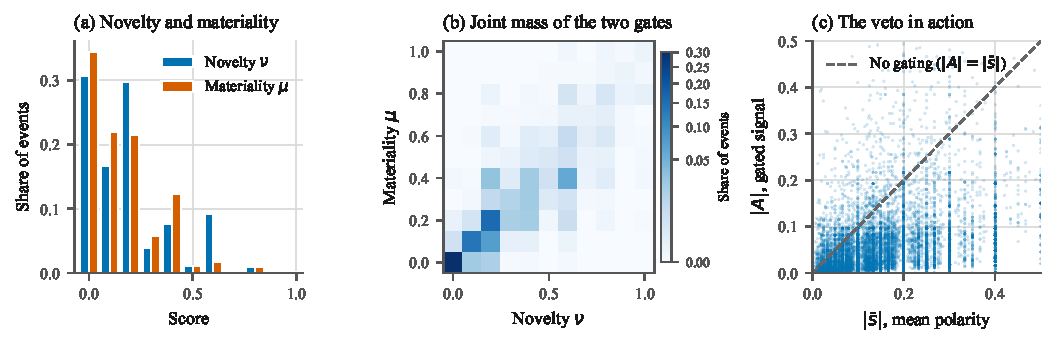
\includegraphics[width=\textwidth]{figures/fig1_axes_veto.pdf}
\caption{The three attributes and the veto they implement, measured on
\ScoredHeadlines\ scored headlines. (a) Marginal distributions of novelty and
materiality; the model reports on a coarse grid, so the honest display is a
discrete bar chart. (b) Joint mass of the two gates, on a power-law colour scale
so the sparse high-novelty, high-materiality cells remain visible. (c) The gated
session aggregate $|A|$ against the mean absolute polarity $|\bar{s}|$ of the
same session: almost every point lies below the 45-degree line, which is
Proposition~\ref{prop:veto} in the data.}
\label{fig:axes}
\end{figure}

\subsection{The screen: does each attribute track its own criterion?}\label{sec:validity}

Each attribute has an external criterion it must track if it measures what it
claims, and neither criterion required further model calls.

\emph{Novelty should track mechanical staleness.} Following the stale-news
literature \citep{tetlock2011}, we measure how much a headline repeats what was
already written about the same ticker: one minus the maximum TF-IDF cosine
similarity to that ticker's headlines over the preceding thirty days. The
comparison set is strictly earlier in time, so the measure is causal and uses no
returns. It is available for $99.9\%$ of headlines (\ScoredForScreen\ of
\HeadlinesScored), with a median of \PriorDocMedian\ prior documents.

\emph{Materiality should track outcome magnitude.} Materiality is defined as the
sensitivity of value to an event \emph{regardless of direction}, so it should
predict the absolute market-adjusted return of the session.

The screen separates the two attributes sharply, but not in the direction the
design needs.

\paragraph{Novelty fails its own criterion.} Figure~\ref{fig:validity}(a) plots
both attributes against deciles of mechanical novelty, and the two curves are the
same curve: parallel, identically shaped, separated by a constant. The
relationship is also non-monotonic, rising from $\NuAtStalest$ at the stalest
decile to $\NuAtPeak$ at decile~\NuPeakDecile\ and then falling to
$\NuAtFreshest$ at the most lexically novel decile --- the model assigns its
\emph{lowest} novelty to the headlines that share least vocabulary with recent
coverage. Controlling for materiality and for the size of the comparison set,
novelty's standardised coefficient on staleness is $\StaleNuBeta$
($t=\StaleNuT$) against materiality's $\StaleMuBeta$ ($t=\StaleMuT$):
distinguishable from zero, but essentially the same number, so novelty carries no
staleness information that materiality does not carry equally. The partial
correlations tell the same story --- $\PartialNuStale$ for novelty given
materiality, $\PartialMuStale$ for materiality given novelty --- as does the
dense subsample with at least twenty prior documents ($\DenseNuStale$ and
$\DenseMuStale$, identical to three decimals). Step~3 of the screen earns its
place here: the raw rank correlation between the novelty attribute and mechanical
novelty is $-0.159$, which read alone would suggest a modest inverse relation
rather than the hump the decile profile actually shows.

\paragraph{Materiality passes its own criterion, decisively.} Over \AbsRetN\
events, a one standard deviation increase in materiality is followed by
$\AbsRetMuBps$ additional basis points of absolute market-adjusted return
($t=\AbsRetMuT$, clustered by date), while novelty enters the same regression
with the \emph{opposite} sign at $\AbsRetNuBps$ basis points ($t=\AbsRetNuT$).
Whatever common factor drives the $0.871$ correlation, the materiality label is
the one that aligns with a real external quantity; conditional on it, the novelty
label points the wrong way (Figure~\ref{fig:validity}(b)).

The verdict is therefore \emph{instrument}, and specifically the novelty
attribute. The model is largely reporting a single latent ``importance''
judgement on two channels; the channel labelled materiality happens to align
with event magnitude, and the channel labelled novelty does not measure novelty
in the sense the design requires.

Step~5 of the screen then supplies the implication that matters most, and
supplies it before any forecasting model exists. The surviving attribute,
materiality, predicts the \emph{magnitude} of the move and not its
\emph{direction} --- exactly what its definition promises. But
Eq.~\eqref{eq:signal} multiplies it into a \emph{directional} signal. A quantity
carrying information about how large a move will be cannot improve a forecast of
which way it will go. That is the cleanest explanation for the materiality
exponent estimating at zero in Section~\ref{sec:exponents}, and it was available
from the screen alone.

\begin{figure}[htbp]
\centering
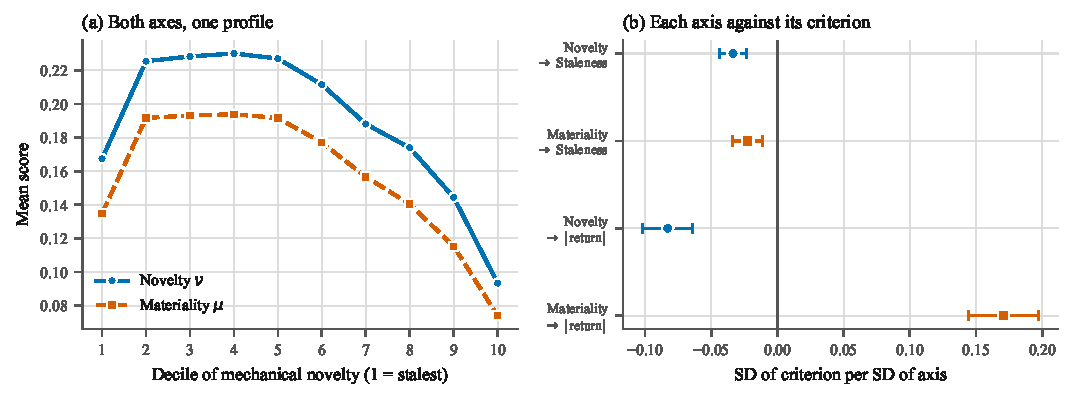
\includegraphics[width=\textwidth]{figures/fig6_convergent_validity.pdf}
\caption{The validity screen. (a) Mean novelty and mean materiality across
deciles of mechanical novelty: the two curves are parallel and identically
shaped, which is what one variable measured twice looks like, and both are
non-monotonic in mechanical novelty. (b) Standardised coefficients of each
attribute on each criterion, in standard deviations of criterion per standard
deviation of attribute, with 95\% intervals from date-clustered standard errors.
Materiality predicts absolute return strongly; novelty does not track mechanical
staleness beyond what materiality already tracks.}
\label{fig:validity}
\end{figure}

\subsection{Predictive content of the aggregators}\label{sec:univariate}

The gated aggregate does predict returns. At the one-session horizon a one
standard deviation move in $A$ is followed by $12.2$ basis points of
market-adjusted return, with a two-way clustered $t$ of $4.14$ and a
Fama--MacBeth $t$ of $3.70$; its rank information coefficient is $0.023$,
averaged over $2{,}548$ trading days with a Newey--West $t$ of $4.44$. At five
sessions the effect is $17.8$ basis points ($t=2.12$) on non-overlapping
windows. By twenty-one sessions nothing survives: every aggregator has
$|t|<0.9$, which is what one expects of headline-level information at a monthly
horizon.

So the text carries signal. The question the study exists to answer is whether
the \emph{product} carries more of it than the recipes it is meant to displace,
and Table~\ref{tab:univariate} says it does not. At one session, mean polarity
earns a \emph{higher} $t$-statistic than the gated aggregate ($5.52$ against
$4.14$); count-weighted polarity produces a larger coefficient still ($14.1$
basis points) and the highest information-coefficient $t$-statistic of the seven
($4.72$); and threshold-filtered polarity --- the recipe a practitioner would
actually deploy --- matches the product almost exactly ($10.0$ basis points).
The information coefficients of the gated aggregate, threshold-filtered polarity
and count-weighted polarity are $0.0230$, $0.0230$ and $0.0228$: identical for
any practical purpose. The one aggregator that clearly underperforms is the
additive combiner $(s+\nu+\mu)/3$ at $3.3$ basis points and $0.010$, which is
worth stating plainly. \emph{Adding} the three attributes is a bad idea, so the
argument against additive combination in Section~\ref{sec:theory} survives; it is
the step from a filter to a product that does not pay.

Figure~\ref{fig:univariate} makes the overlap visible. At the horizons where
anything is estimable, the confidence intervals of all seven aggregators sit on
top of one another.

\begin{table}[htbp]
\caption{Predictive regressions of forward market-adjusted returns on each
aggregator, one aggregator at a time. Regressors are standardised, so a
coefficient reads as basis points of forward return per one standard deviation of
signal. Standard errors are two-way clustered by date and symbol; horizons beyond
one session use non-overlapping windows. Stars mark significance at the 10\%,
5\% and 1\% levels.}
\label{tab:univariate}
\begin{tabular}{@{}lcccccc@{}}
\toprule
 & \multicolumn{2}{c}{$H=1$} & \multicolumn{2}{c}{$H=5$} & \multicolumn{2}{c}{$H=21$} \\
Aggregator & bps & $t$ & bps & $t$ & bps & $t$ \\
\midrule
Gated signal $A$ & 12.2$^{***}$ & 4.14 & 17.8$^{**}$ & 2.12 & 11.7 & 0.60 \\
Relevance-filtered polarity & 10.0$^{***}$ & 5.11 & 12.5$^{*}$ & 1.82 & 10.4 & 0.46 \\
Mean polarity & 9.3$^{***}$ & 5.52 & 13.6$^{**}$ & 2.03 & 18.5 & 0.87 \\
Count-weighted polarity & 14.1$^{***}$ & 4.78 & 17.1$^{**}$ & 2.29 & 14.3 & 0.62 \\
Additive combiner & 3.3$^{***}$ & 3.82 & 3.9 & 0.71 & -3.3 & -0.16 \\
Novelty gate only ($s\nu$) & 11.1$^{***}$ & 4.71 & 15.8$^{**}$ & 2.14 & 7.3 & 0.38 \\
Materiality gate only ($s\mu$) & 11.9$^{***}$ & 4.53 & 15.1$^{*}$ & 1.89 & 10.8 & 0.60 \\
\botrule
\end{tabular}
\footnotetext{Largest estimation sample: 48,260 symbol-sessions.}
\end{table}


\begin{figure}[htbp]
\centering
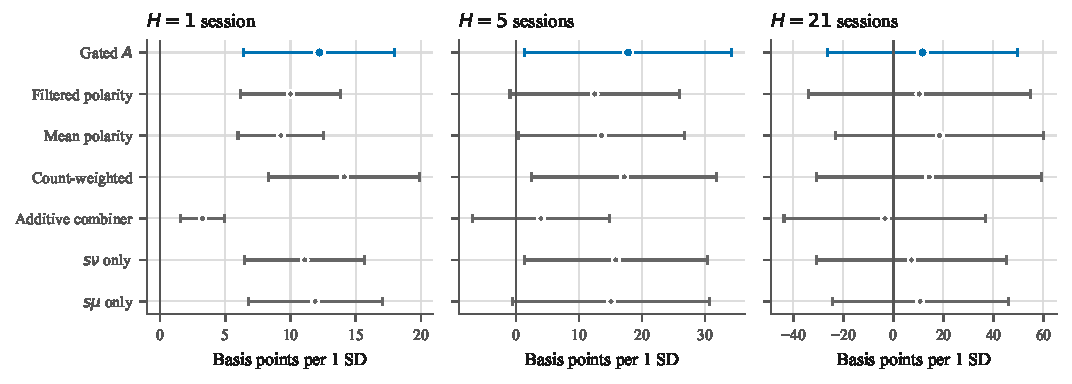
\includegraphics[width=\textwidth]{figures/fig2_univariate.pdf}
\caption{Forward-return coefficient on each aggregator, in basis points per one
standard deviation of signal, with 95\% intervals from two-way clustered
standard errors. The gated signal is highlighted; the alternatives are shown in
neutral ink.}
\label{fig:univariate}
\end{figure}

\subsection{The nested horse race}\label{sec:horserace}

Entering all four terms together (Table~\ref{tab:horserace}) was intended to be
the sharp test: multiplicative gating predicts that the product loads and
absorbs the lower-order terms. What happens instead is that nothing is
individually identified. At one session the gated aggregate carries the largest
coefficient ($16.3$ basis points) but only $t=1.58$, while mean polarity falls to
$t=1.26$ and the two single-gate ablations take opposite signs. At five and
twenty-one sessions the coefficients grow large and alternate in sign ---
$+50.3$ for the product against $-36.2$ for the materiality gate at five
sessions --- with $|t|<2$ throughout.

This pattern is diagnostic of collinearity, not of a hidden effect, and
Section~\ref{sec:descriptive} already said why: with $\nu$ and $\mu$ correlated
at $0.871$ and all four regressors built from the same polarity, the design
matrix is close to singular and the individual coefficients are not separately
estimable. We therefore decline to read anything into the sign or size of any
single term. The honest conclusion is a statement about what the data
\emph{cannot} answer: on this corpus the nested horse race lacks the power to
distinguish the product from its components.

\begin{table}[htbp]
\caption{The nested horse race. All four terms enter one regression, so each
coefficient is the marginal contribution of that term given the others.
Multiplicative gating predicts that the gated signal loads and absorbs the
lower-order terms. Regressors standardised; two-way clustered $t$-statistics.}
\label{tab:horserace}
\begin{tabular}{@{}lcccccc@{}}
\toprule
 & \multicolumn{2}{c}{$H=1$} & \multicolumn{2}{c}{$H=5$} & \multicolumn{2}{c}{$H=21$} \\
Term & bps & $t$ & bps & $t$ & bps & $t$ \\
\midrule
Mean polarity & 6.2 & 1.26 & 23.1$^{*}$ & 1.92 & 85.5$^{*}$ & 1.76 \\
Novelty gate only ($s\nu$) & -9.1 & -1.30 & -15.2 & -0.63 & -103.8$^{*}$ & -1.77 \\
Materiality gate only ($s\mu$) & 0.4 & 0.05 & -36.2 & -1.25 & -64.7 & -0.59 \\
Gated signal $A$ & 16.3 & 1.58 & 50.3 & 1.33 & 111.8 & 0.98 \\
\botrule
\end{tabular}
\end{table}


\subsection{Free exponents}\label{sec:exponents}

The horse race cannot separate the terms, but the exponent grid asks a cleaner
question, because it varies the functional form directly instead of trying to
identify collinear regressors. Remark~\ref{rem:notpinned} left $\alpha$ and
$\beta$ free; here we estimate them by sweeping $s\,\nu^{\alpha}\mu^{\beta}$ over
a grid of \GridPerHorizon\ points on $[0,2]^2$ and reading off the information
coefficient of the resulting aggregate.

The answer is unambiguous and it is not the one the unit-exponent product
predicts. At one session the grid maximum sits at $\alpha=\BestAlphaHOne$,
$\beta=\BestBetaHOne$ with information coefficient $\BestICHOne$: the materiality
exponent is estimated at \emph{exactly zero}, as Step~5 of the screen implied it
would be. The unit-exponent product assumed by Eq.~\eqref{eq:signal} scores
$\UnitICHOne$, and switching the gates off altogether --- $\alpha=\beta=0$, which
collapses the aggregate to plain mean polarity --- scores $\PureICHOne$. At five
sessions the maximum \emph{is} the no-gating corner, $\alpha=\beta=0$ with
$\BestICHFive$, against $\UnitICHFive$ for the unit-exponent product: there,
gating is not merely unhelpful but actively harmful.

Two conclusions follow. First, $H_0\!:\alpha=\beta=1$ is rejected, and rejected
in the direction of the null model rather than toward some richer weighting.
Second, and more important for a team deciding where to spend effort, the entire
surface spans only $0.0201$ to $0.0225$ in information coefficient
(Figure~\ref{fig:exponents}). The objective is nearly flat in the exponents, so
the choice of gating weights --- including the choice not to gate --- moves
predictive accuracy by an amount small relative to its own sampling error. That
flatness, rather than the location of any maximum, is the finding, and it is why
every comparison in Section~\ref{sec:selective} lands inside its confidence
interval.

\begin{figure}[htbp]
\centering
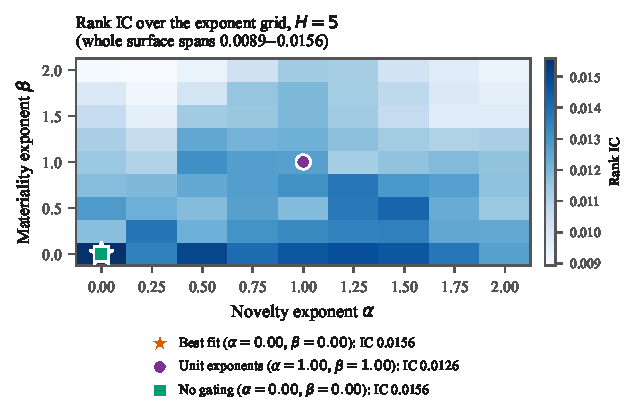
\includegraphics[width=0.62\textwidth]{figures/fig4_exponents.pdf}
\caption{Information coefficient of the aggregate built from
$s\,\nu^{\alpha}\mu^{\beta}$ over a grid of exponents. The unit-exponent product
assumed by Eq.~\eqref{eq:signal} is marked, as is the empirical maximum;
Remark~\ref{rem:notpinned} explains why the axioms leave this an open question.}
\label{fig:exponents}
\end{figure}

\subsection{Selective forecasting with and without the gated signal}\label{sec:selective}

This is the experiment the design has to pass: the conviction gate is fitted
twice on identical walk-forward folds, once on price features alone and once on
price features plus the gated text signal, and the reported quantity is the
difference.

There is no difference. Adding $A$ moves precision at a fixed $10\%$ coverage by
$\GapPriceHOne$ percentage points at one session
(95\% CI \GapPriceCIHOne, $p=\GapPricePHOne$), $\GapPriceHFive$ points at five
sessions (\GapPriceCIHFive, $p=\GapPricePHFive$) and $\GapPriceHTwentyOne$ points
at twenty-one (\GapPriceCIHTwentyOne, $p=\GapPricePHTwentyOne$). Against
threshold-filtered polarity rather than against price alone the gaps are
$\GapRelfHOne$, $\GapRelfHFive$ and $\GapRelfHTwentyOne$ points. Every interval
contains zero, and the point estimates change sign across horizons. The
risk--coverage curves of Figure~\ref{fig:riskcov} say the same thing without
reference to any threshold: the curves for the four feature sets are
indistinguishable over the whole coverage range, and their AURCs differ in the
third decimal.

One result in Table~\ref{tab:gate} does not fit the pattern, and we report it
because it is the most interesting thing in the table. The \emph{text-only} model
--- no price features at all --- achieves the best AURC at both short horizons
($\AurcAHOne$ against $\AurcPriceHOne$ for price-only at one session, and $0.468$
against $\AurcPriceHFive$ at five) and the best precision at five sessions
($55.3\%$ against $\PrecPriceHFive\%$ for price-only, on a $\BaseRateHFive\%$
base rate). The headlines therefore carry decision-relevant information that the
price features do not, and a learner given the text alone finds it. What the
learner cannot do is exploit that information \emph{once price features are also
available}: the combined model is no better than price alone. Whether this
reflects genuine redundancy or a failure of the gradient-boosted learner to
allocate capacity to a weak, sparse feature beside strong dense ones, we cannot
determine from these data, and we would not want a reader to take the first
explanation for granted.

\begin{table}[htbp]
\caption{Selective forecasting with and without the gated text signal. Precision
is the realised up-rate of the most confident 10\% of out-of-sample predictions,
a fixed coverage that makes the variants comparable without reference to any
tuned threshold; AURC is the area under the risk--coverage curve, for which lower
is better. All figures are pooled over walk-forward test years. The lower panel
bootstraps the precision gap by resampling whole dates.}
\label{tab:gate}
\small
\begin{tabular}{@{}lcccccc@{}}
\toprule
 & \multicolumn{2}{c}{$H=1$} & \multicolumn{2}{c}{$H=5$} & \multicolumn{2}{c}{$H=21$} \\
Feature set & Prec. & AURC & Prec. & AURC & Prec. & AURC \\
\midrule
Price $+$ gated signal $A$ & 51.5 & 0.479 & 52.4 & 0.472 & 59.7 & 0.458 \\
Price $+$ filtered polarity & 51.4 & 0.482 & 53.8 & 0.472 & 59.1 & 0.460 \\
Price $+$ mean polarity & 51.2 & 0.484 & 53.4 & 0.470 & 59.3 & 0.459 \\
Price only & 51.2 & 0.485 & 54.0 & 0.473 & 59.0 & 0.457 \\
Text only & 52.8 & 0.479 & 55.3 & 0.468 & 58.9 & 0.462 \\
\midrule
Always-up base rate & \multicolumn{2}{c}{51.8\%} & \multicolumn{2}{c}{53.3\%} & \multicolumn{2}{c}{54.9\%} \\
\botrule
\end{tabular}

\vspace{0.6em}
\begin{tabular}{@{}lccc@{}}
\toprule
Precision gap at 10\% coverage & Estimate (pp) & 95\% CI & $p$ \\
\midrule
$H=1$, vs.\ price only & +0.37 & [-1.26, +1.96] & 0.685 \\
$H=1$, vs.\ filtered polarity & +0.07 & [-1.70, +1.83] & 0.938 \\
$H=1$, vs.\ mean polarity & -0.05 & [-2.23, +2.14] & 0.948 \\
$H=5$, vs.\ price only & -1.23 & [-3.52, +1.13] & 0.322 \\
$H=5$, vs.\ filtered polarity & -0.83 & [-3.10, +1.40] & 0.482 \\
$H=5$, vs.\ mean polarity & -0.65 & [-2.96, +1.64] & 0.587 \\
$H=21$, vs.\ price only & +0.01 & [-0.74, +0.72] & 1.000 \\
$H=21$, vs.\ filtered polarity & +0.37 & [-0.23, +0.97] & 0.252 \\
$H=21$, vs.\ mean polarity & +0.28 & [-0.32, +0.84] & 0.345 \\
\botrule
\end{tabular}
\end{table}


\begin{figure}[htbp]
\centering
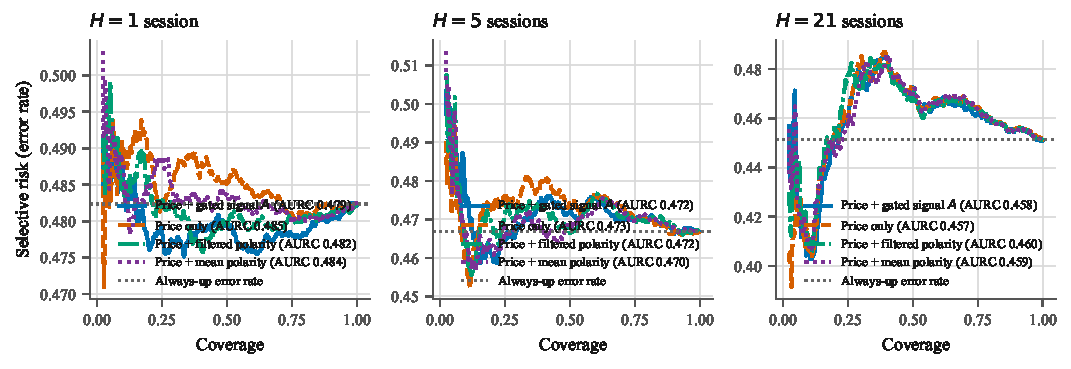
\includegraphics[width=\textwidth]{figures/fig3_risk_coverage.pdf}
\caption{Risk--coverage curves for the walk-forward selective forecaster. Each
curve traces the error rate accepted at every coverage level, so the comparison
does not depend on the choice of any single conviction threshold; the area under
each curve (AURC, lower is better) appears in the legend.}
\label{fig:riskcov}
\end{figure}

\subsection{Deployment evidence: coverage and calibration}\label{sec:live}

The results above concern the text stage. The decision stage was studied on the
production system, where the evidence is of a different kind: not whether a
signal predicts, but whether a system in operation tells the truth about its own
uncertainty.

It did not. Between 19 April and 12 June 2026 the system issued and later
resolved 621 price-interval forecasts on seven large caps, each carrying a
nominal $90\%$ interval with a median half-width of $5.6\%$ of price. Had those
intervals been calibrated, about $90\%$ would have contained the realised price;
empirical coverage was $70.7\%$, a $19.3$ percentage-point shortfall
(Table~\ref{tab:live}, Figure~\ref{fig:deployment}(a)). Most forecasts sat at the
ten-day horizon, where coverage was $69.2\%$ over 575 resolved forecasts. Nothing
in the pipeline noticed, which is the point: overconfidence is silent unless
somebody scores it.

The directional head failed in the same direction and for a diagnosable reason.
It reported next-day up-probabilities clustered near $0.80$ against a realised
accuracy near $0.51$, giving an expected calibration error of $0.345$ and a Brier
score above $0.366$ --- worse than predicting $0.5$ every time. The cause was the
stacking domain mismatch of Section~\ref{sec:calib}, and the three-stage repair
cut expected calibration error from $0.345$ to $0.049$ while leaving accuracy
untouched. Calibration changed what the model \emph{said about its confidence},
not what it predicted, which is precisely the distinction the design insists on.

With probabilities pulled back to the base rate, the walk-forward conviction gate
on the 54-name deployment universe (2018--2026, 91{,}471 training rows and
50{,}272 out-of-sample rows) settles at $\tau^\star=0.63$ and fires on $5.6\%$ of
observations, abstaining on the rest. The fired bucket realises $60.6\%$
directional precision against a $58.0\%$ always-up base rate over $2{,}840$
pooled calls: a $2.6$ point edge with a $95\%$ binomial interval of $58.8$ to
$62.4\%$. We do not over-read it. Per-year counts are small, the swing from
$+10.8$ points in 2025 to $-2.4$ in 2024 is within sampling noise
(Figure~\ref{fig:deployment}(b)), and the ranking area under the curve is about
$0.47$, so what edge exists lives in the high-conviction tail and not in the
ordering. Crucially for this paper, \emph{that gate contains no text feature at
all}: it is evidence that calibrated abstention is worth building, not evidence
for the decomposition.

\begin{table}[htbp]
\caption{Deployment evidence from the live forecast ledger. Every interval
carries a nominal 90\% level. Panel B reports the walk-forward conviction gate on
the 54-name deployment universe, where precision is the realised up-rate of the
fired high-conviction bucket and the base is the unconditional always-up rate.}
\label{tab:live}
\begin{tabular}{@{}lccc@{}}
\toprule
\multicolumn{4}{@{}l}{\textit{Panel A: interval coverage by horizon}} \\
Horizon & Resolved forecasts & Nominal & Empirical \\
\midrule
5 trading days  & 8   & 90.0\% & 100.0\% \\
10 trading days & 575 & 90.0\% & 69.2\%  \\
20 trading days & 38  & 90.0\% & 86.8\%  \\
\textbf{All}    & \textbf{621} & \textbf{90.0\%} & \textbf{70.7\%} \\
\botrule
\end{tabular}

\vspace{0.6em}
\begin{tabular}{@{}lcccc@{}}
\toprule
\multicolumn{5}{@{}l}{\textit{Panel B: walk-forward conviction gate by test year}} \\
Test year & Fires & Fired precision & Always-up base & Edge (pp) \\
\midrule
2022 & 365 & 61.6\% & 54.0\% & $+7.6$ \\
2023 & 290 & 68.3\% & 65.3\% & $+3.0$ \\
2024 & 932 & 53.3\% & 55.7\% & $-2.4$ \\
2025 & 822 & 69.0\% & 58.2\% & $+10.8$ \\
2026 & 431 & 54.5\% & 47.1\% & $+7.4$ \\
\textbf{Pooled} & \textbf{2{,}840} & \textbf{60.6\%} & \textbf{58.0\%} & \textbf{$+2.6$} \\
\botrule
\end{tabular}
\footnotetext{The pooled base is the unconditional always-up rate over all
out-of-sample rows, not the fires-weighted mean of the yearly bases (55.9\%); the
pooled edge is therefore the more conservative of the two comparisons.}
\end{table}


\begin{figure}[htbp]
\centering
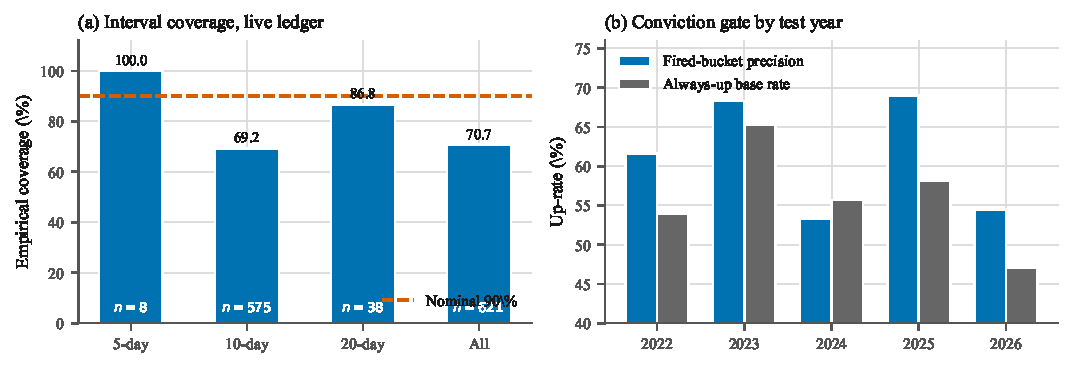
\includegraphics[width=\textwidth]{figures/fig5_deployment.pdf}
\caption{Deployment evidence. (a) Empirical coverage of nominal 90\% price
intervals on the live ledger, by horizon. (b) Fired-bucket precision of the
conviction gate against the always-up base rate, by walk-forward test year, at
roughly a 5.6\% firing rate.}
\label{fig:deployment}
\end{figure}

\subsection{Robustness}\label{sec:robust}

A null result is only worth reporting if it is not an artefact of the analyst's
choices, so we varied the three that matter, in \RobustnessFits\ re-estimations.

\emph{The materiality floor.} Sweeping $\mu_0$ from $0$ (no floor) to $0.40$
leaves the one-session coefficient on $A$ between $12.0$ and $12.2$ basis points
with $t$ between $3.97$ and $4.14$. The floor does not bind on the conclusion,
which is what one expects when the exponent on materiality is estimated at zero.
One detail cuts the other way and we note it: at five sessions the information
coefficient rises from $0.013$ at $\mu_0=0$ to $0.025$ at $\mu_0=0.25$ and above,
with the Newey--West $t$ going from $1.24$ to $2.25$. A \emph{hard threshold
filter} thus helps where multiplicative weighting does not --- consistent with
the exponent surface, and consistent with what practitioners already do with
vendor relevance scores.

\emph{Overlapping versus non-overlapping windows.} Using every session rather
than every $H$-th weakens the five-session result from $17.8$ basis points
($t=2.12$) to $8.9$ ($t=1.68$), in the direction the overlapping-observation
literature predicts. We report non-overlapping windows as the primary
specification for that reason; neither choice changes the comparison between
aggregators, which is what the study turns on.

\emph{Quiet sessions.} Restricting the panel to symbol-sessions carrying scored
news is the primary specification, since including quiet sessions pads the sample
with rows where every text aggregator is identically zero and can only dilute any
difference between them.

\emph{Repeatability of the instrument.} Cross-model agreement is reported in
Section~\ref{sec:reliability}. We regard it as the weakest link in the
measurement chain and the first thing a replication should attack.

% =============================================================================
\section{Discussion}\label{sec:discussion}
% =============================================================================

\subsection{Why the decomposition did not pay}

Section~\ref{sec:validity} lets us be specific rather than speculative, and the
answer has two parts.

\emph{One attribute is not measuring what it is named.} Novelty fails its
external criterion: it does not track mechanical staleness beyond what
materiality already tracks, its profile against mechanical novelty is the same
curve as materiality's, and it is non-monotonic besides. Materiality passes
decisively, predicting absolute market-adjusted returns at $\AbsRetMuT$ standard
errors. So the $0.871$ correlation is not the world telling us that novel news is
material news; it is one latent importance judgement reported twice under two
labels, only one of which corresponds to something external. A product of two
gates cannot behave like a two-gate product when only one gate exists.

\emph{The surviving attribute carries the wrong quantity for the task.}
Materiality is by definition about magnitude irrespective of sign, and that is
exactly how it behaves. Multiplying it into a \emph{signed} signal, as
Eq.~\eqref{eq:signal} does, asks a magnitude variable to sharpen a direction
forecast, which it has no means of doing. This is the cleanest reading of the
zero materiality exponent, and it points somewhere constructive: the same
decomposition aimed at a volatility or absolute-return target, where
materiality's information is of the relevant kind, is a genuinely different
experiment and one we have not run.

\emph{Attenuation remains a live secondary concern.} Cross-model intraclass
correlations are $\ICCS$ for polarity but only $\ICCNu$ for novelty, and the
product inherits $0.601$; multiplying noisy factors compounds their noise, so
classical errors-in-variables would bias the measured contribution of gating
toward zero. We cannot rule this out, and it is a further reason the design
deserves a rematch with a better instrument rather than a dismissal. What it does
not license is treating the null as a measurement artefact by assumption --- and
in any case attenuation cannot explain why novelty points the \emph{wrong way} on
absolute returns, which is a validity failure and not a noise problem.

Note also what survived. The additive combiner performed worst of all the
aggregators, so collapsing the attributes by addition is clearly wrong; and a
\emph{hard} materiality filter improved the five-session information coefficient
from $0.013$ to $0.025$ where multiplicative weighting did not. Read together,
these say that relevance information is worth using as a \emph{filter} --- decide
which items to look at --- but not as a continuous multiplicative \emph{weight}
on the ones that survive. The practitioner convention of thresholding a vendor
relevance score, which we set out to improve on, appears to be the right call.

\subsection{What the screen would have saved}\label{sec:saved}

The value of a screen is not that it produces a result but that it produces the
result \emph{early}, and Table~\ref{tab:cost} is the accounting. Every finding in
Section~\ref{sec:results} is an implication of the screen's two regressions:

\begin{itemize}
\item \emph{Novelty and materiality collapse into one attribute} $\Rightarrow$
  the nested horse race cannot identify separate terms
  (Section~\ref{sec:horserace}), and the exponent surface is nearly flat
  (Section~\ref{sec:exponents}).
\item \emph{The surviving attribute measures magnitude, not direction}
  $\Rightarrow$ the materiality exponent estimates at zero against a signed
  target (Section~\ref{sec:exponents}).
\item \emph{Neither implication leaves room for an incremental gate}
  $\Rightarrow$ the selective forecaster with and without $A$ differs by less
  than its own sampling error (Section~\ref{sec:selective}).
\end{itemize}

The three screen objects and the \DownstreamTotal\ downstream objects are not
comparable in machine time; a modern laptop runs both. They are comparable in the
resource that actually binds an analytics team, which is the sequence of
decisions an analyst makes while a result is still ambiguous. Each of the
\GridTotal\ exponent evaluations, \UnivariateFits\ predictive regressions and
\GateFits\ walk-forward fits carries a specification choice --- which horizon is
primary, whether to report overlapping windows, which threshold defines coverage
--- and each such choice is an opportunity for a result to be nudged toward the
one the analyst hoped for. Running the screen first removes the ambiguity that
makes those choices consequential.

\subsection{Managerial implications}\label{sec:managerial}

For a team that is about to build on multi-attribute language-model scores, the
findings translate into four specific rules.

\begin{enumerate}
\item \textbf{Treat every prompted attribute as an instrument requiring
  validation, not as a column requiring monitoring.} Existing feature-store
  controls --- drift, missingness, range --- are all passed by an attribute that
  measures the wrong construct. Add a validity gate at feature onboarding, and
  make an attribute's criterion a mandatory field in its specification.
\item \textbf{Require the criterion to be named before the scores are
  generated.} A criterion chosen after inspecting the scores is a rationalisation.
  The version of this study that we would defend is the one in which each
  attribute's criterion was fixed by its definition: novelty against staleness,
  materiality against outcome magnitude.
\item \textbf{Budget attributes by validated count, not requested count.} The
  marginal cost of an extra attribute in the prompt is near zero, but the
  marginal cost of an \emph{unvalidated} extra attribute is the entire modelling
  programme built on it. In this study the ratio was \ScreenTotal\ objects to
  \DownstreamTotal.
\item \textbf{Use relevance as a filter, not as a weight.} Where the two are
  distinguishable in these data, the hard threshold wins: it lifted the
  five-session information coefficient from $0.013$ to $0.025$ where continuous
  multiplicative weighting moved nothing. This is a rare case of the simpler
  incumbent practice being vindicated against a more elaborate proposal.
\end{enumerate}

There is also a negative recommendation. The most reusable part of the screen is
step~5 --- checking that the criterion is the right \emph{kind} of quantity for
the task --- and it is the step most easily skipped, because it feels like
philosophy rather than measurement. It was the step that predicted the single
most consequential number in the study, the zero materiality exponent, and it
costs nothing but a sentence of thought per attribute.

\subsection{Scope beyond this application}

Nothing in Section~\ref{sec:theory} is specific to equities. Any stream of
timestamped textual events feeding a decision has the same structure, and the
same failure mode when conceptually distinct attributes are requested from one
prompt: triage of clinical alerts, operations tickets and content-moderation
queues all ask how bad, how new and how consequential, and all are exposed to a
model that answers the three questions with one judgement. The screen transfers
directly, because its only requirement is that each attribute admit an observable
criterion the others have no reason to track --- for a ticket-urgency attribute,
time-to-resolution; for a moderation-severity attribute, the eventual enforcement
action.

The decision-stage half of the design is an instance of selective classification
\citep{chow1970,geifman2017}, here paired with a probability whose calibration was
repaired rather than assumed, and the interval-coverage failure of
Section~\ref{sec:live} is exactly the problem distribution-free methods
\citep{angelopoulos2023} are built for.

\subsection{Limitations}\label{sec:limits}

Five limitations bound what may be concluded, and we would rather state them than
have them found.

\emph{The validation market is not the deployment market.} The decomposition is
tested on US headlines while the production system operates on Indian equities.
We report no result that crosses that boundary, but a reader should not read the
US panel as evidence about the NSE's microstructure, disclosure regime or news
supply, all of which differ.

\emph{The attributes are judgements, and one of them did not survive
validation.} Anchoring the prompt tightens the scores and
Section~\ref{sec:reliability} quantifies their repeatability, but repeatability
is not validity: a scorer can be perfectly consistent and consistently wrong,
which is close to what the screen finds for novelty. Every result about gating is
therefore a joint test of the design and of this particular instrument, and a
differently worded rubric, a larger model, or a two-stage prompt that scores the
attributes independently might separate them where ours did not. We consider that
the single most valuable follow-up.

\emph{The external criteria are proxies.} Lexical similarity over a thirty-day
window is a serviceable but crude stand-in for what the market already knew, and
absolute return is a noisy realisation of an event's true importance. A criterion
failure is therefore weaker evidence than a criterion success: materiality
passing is strong evidence it measures something, whereas novelty failing is
consistent with both a bad attribute and a bad proxy.

\emph{The comparison is against feasible baselines, not against a vendor feed.}
The most informative comparison would be against a commercial relevance and
novelty product on the same headlines. We do not have a licence for one, so
threshold-filtered polarity is our best available stand-in for what a
practitioner would deploy.

\emph{Selection and multiple testing.} We report several horizons, several
aggregators and several feature sets. The risk--coverage curves and the
non-overlapping-window specification remove the most common sources of optimism,
and differences between models carry bootstrap intervals, but a reader who wants
a single number with a family-wise guarantee should apply a stepdown correction
\citep{romano2005} to the horse-race column and read the result accordingly.
Applied machine learning in this domain has a well-documented tendency to
discover edges that do not survive \citep{bailey2017,harvey2016}, and we would
rather our estimates be read with that prior in mind.

% =============================================================================
\section{Conclusions}\label{sec:conclusion}
% =============================================================================

A textual event carries direction, surprise and consequence, and there is a clean
argument that these should combine multiplicatively: the product makes freshness
and relevance preconditions for influence, it caps the signal at its weakest
factor, and under continuity, monotonicity and ratio-scale separability it is the
form the attributes must take, up to exponents the axioms leave free.

Measured against real data, the argument does not pay. On \ScoredHeadlines\
headlines covering \NCompanies\ companies, the gated aggregate predicts
market-adjusted returns at short horizons but no better than mean polarity,
count-weighted polarity or threshold-filtered polarity; estimating the exponents
freely puts materiality's at zero and, at five sessions, collapses the aggregate
to plain polarity; and adding the gated signal to a walk-forward selective
forecaster moves precision at fixed coverage by between $-1.2$ and $+0.4$
percentage points, with every interval containing zero.

The explanation is in the measurement rather than in the market. Novelty and
materiality, as an instruction-tuned model scores them, correlate at $0.871$;
validated against external criteria, only materiality survives, predicting
absolute market-adjusted returns at $\AbsRetMuT$ standard errors, while novelty
fails to track mechanical staleness beyond what materiality already tracks and
enters absolute returns with the wrong sign. The three-attribute decomposition is
empirically a two-attribute one, and the attribute that does measure something
measures \emph{magnitude}, which a signed product has no way to exploit.

Two things survive as positive findings. Adding the attributes is worse than
multiplying them, so the case against additive combination stands. And using
relevance as a hard filter rather than a continuous weight improves the
five-session information coefficient from $0.013$ to $0.025$ --- which is what
practitioners already do with vendor relevance scores, now with evidence behind
it. Separately, on the deployment side, nominal $90\%$ intervals covered $70.7\%$
of live outcomes, a three-stage recalibration cut expected calibration error from
$0.345$ to $0.049$ without touching accuracy, and a conviction gate abstaining on
$94\%$ of names raised the thirty-day hit rate to $60.6\%$ against a $58.0\%$
base --- evidence that calibrated abstention is worth building, independent of
anything the text stage does.

The managerial conclusion is the ratio. The modelling programme that established
all of the above comprised \DownstreamTotal\ fitted objects. The screen that
implied all of it comprised \ScreenTotal, used no labelled data, and added
\ScreenModelCalls\ calls to the scoring model. As multi-attribute prompting
spreads through analytics pipelines, the constraint on feature quality will not
be the cost of generating attributes; it will be the discipline to check that the
attributes generated are the ones that were asked for. Two experiments follow
directly from this one and neither is run here: an instrument whose novelty
channel passes an external validity check would give the design the fair test it
has not yet had, and pointing the same decomposition at a volatility or
absolute-return target asks the question the signed formulation cannot. The
measurements reported here are designed to make both possible.

% =============================================================================
\section*{Declarations}

\paragraph{Funding} No external funding was received for this work.

\paragraph{Competing interests} The authors declare no competing interests.

\paragraph{Ethics approval} Not applicable. The study uses public news and price
data and involves no human subjects.

\paragraph{CRediT authorship contribution statement}
\ifblind
Author contributions are withheld for double-blind review and will be supplied
on acceptance.
\else
\textbf{Anandkumar Pardeshi:} Conceptualization, Methodology, Software, Formal
analysis, Investigation, Data curation, Writing --- original draft,
Visualization. \textbf{Sujata Deshmukh:} Conceptualization, Methodology,
Validation, Writing --- review \& editing, Supervision. Both authors read and
approved the final manuscript.
\fi

\paragraph{Declaration of generative AI in scientific writing}
An instruction-tuned language model is used as a measurement instrument
\emph{within the system under study}, scoring headlines along the three
attributes from the anchored rubric of Section~\ref{sec:scoring}; those outputs
are persisted for audit. During manuscript preparation a large language model was
used solely to improve language and readability. No generative tool produced the
data, results, figures or interpretations, and the authors take full
responsibility for the content of the publication.

\paragraph{Data availability} The FNSPID news corpus is publicly available
\citep{dong2024}; price data are public end-of-day records. The scored attribute
values, the derived panel, the analysis code and the production forecast ledger
underlying the reported tables and figures are available from the corresponding
author on reasonable request.

\ifblind
\else
\paragraph{Acknowledgements} The authors thank Fr.~C.~Rodrigues Institute of
Technology for computing support.

\paragraph{Author ORCIDs}
Anandkumar Pardeshi \textemdash\ \url{https://orcid.org/0000-0003-2806-3305};
Sujata Deshmukh \textemdash\ \url{https://orcid.org/0000-0001-9893-6947}.
\fi

\bibliographystyle{elsarticle-harv}
\bibliography{refs}

\end{document}
